% Created by tikzDevice version 0.12.5 on 2023-10-01 18:55:02
% !TEX encoding = UTF-8 Unicode
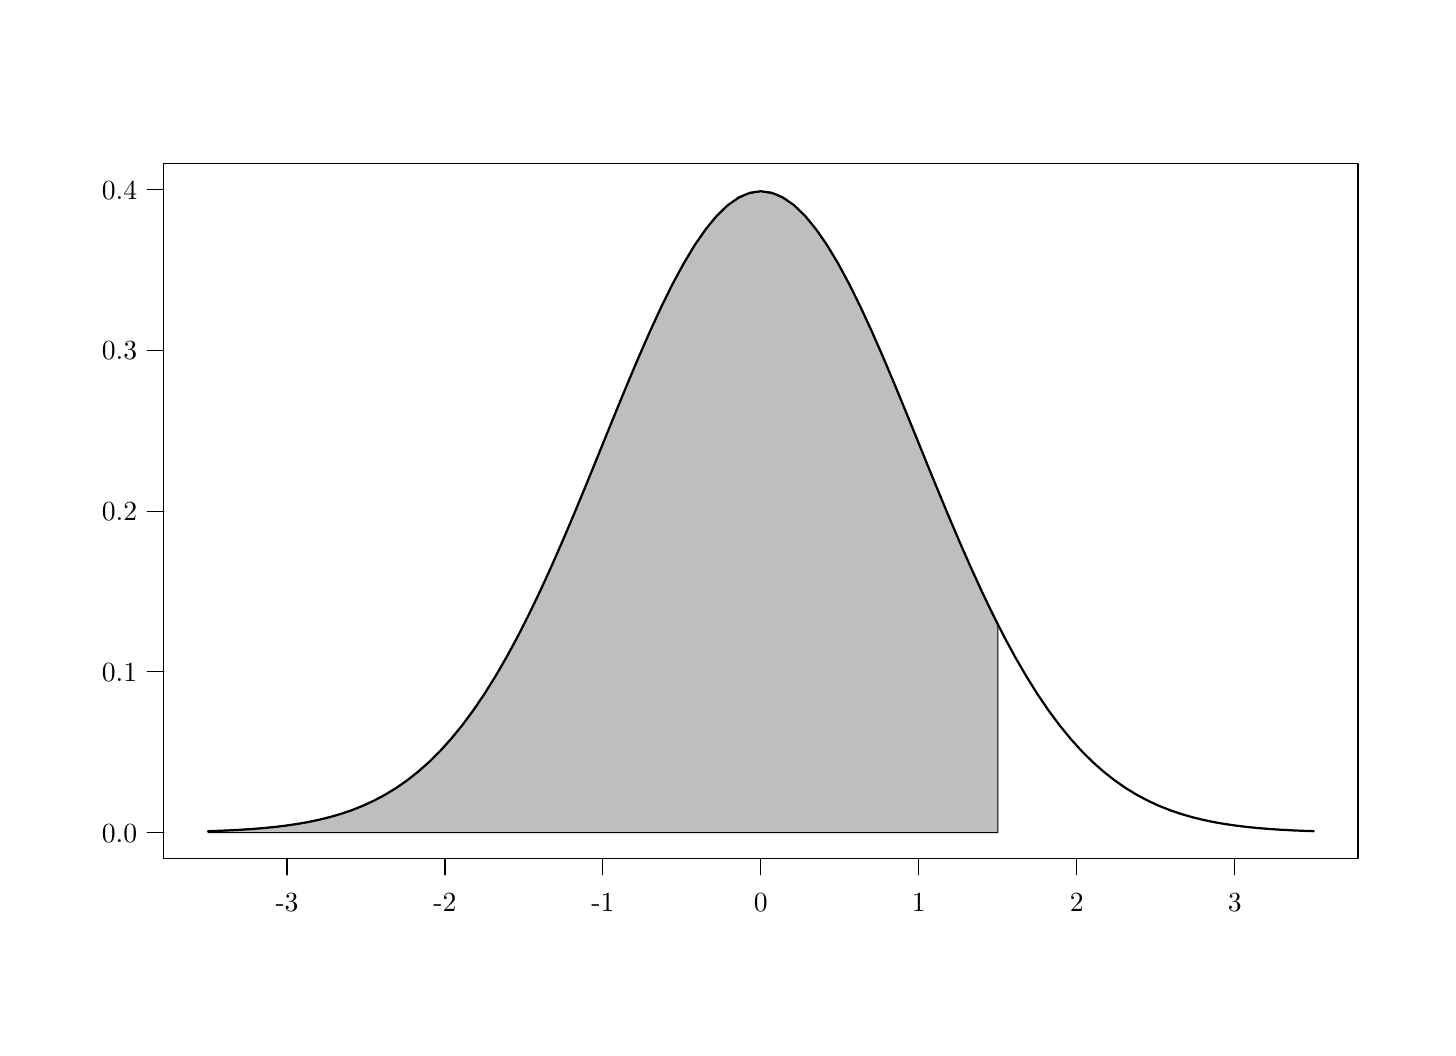
\begin{tikzpicture}[x=1pt,y=1pt]
\definecolor{fillColor}{RGB}{255,255,255}
\path[use as bounding box,fill=fillColor,fill opacity=0.00] (0,0) rectangle (505.89,361.35);
\begin{scope}
\path[clip] (  0.00,  0.00) rectangle (505.89,361.35);
\definecolor{drawColor}{RGB}{0,0,0}

\path[draw=drawColor,line width= 0.4pt,line join=round,line cap=round] ( 93.72, 61.20) -- (436.17, 61.20);

\path[draw=drawColor,line width= 0.4pt,line join=round,line cap=round] ( 93.72, 61.20) -- ( 93.72, 55.20);

\path[draw=drawColor,line width= 0.4pt,line join=round,line cap=round] (150.79, 61.20) -- (150.79, 55.20);

\path[draw=drawColor,line width= 0.4pt,line join=round,line cap=round] (207.87, 61.20) -- (207.87, 55.20);

\path[draw=drawColor,line width= 0.4pt,line join=round,line cap=round] (264.94, 61.20) -- (264.94, 55.20);

\path[draw=drawColor,line width= 0.4pt,line join=round,line cap=round] (322.02, 61.20) -- (322.02, 55.20);

\path[draw=drawColor,line width= 0.4pt,line join=round,line cap=round] (379.10, 61.20) -- (379.10, 55.20);

\path[draw=drawColor,line width= 0.4pt,line join=round,line cap=round] (436.17, 61.20) -- (436.17, 55.20);

\node[text=drawColor,anchor=base,inner sep=0pt, outer sep=0pt, scale=  1.00] at ( 93.72, 42.00) {-3};

\node[text=drawColor,anchor=base,inner sep=0pt, outer sep=0pt, scale=  1.00] at (150.79, 42.00) {-2};

\node[text=drawColor,anchor=base,inner sep=0pt, outer sep=0pt, scale=  1.00] at (207.87, 42.00) {-1};

\node[text=drawColor,anchor=base,inner sep=0pt, outer sep=0pt, scale=  1.00] at (264.94, 42.00) {0};

\node[text=drawColor,anchor=base,inner sep=0pt, outer sep=0pt, scale=  1.00] at (322.02, 42.00) {1};

\node[text=drawColor,anchor=base,inner sep=0pt, outer sep=0pt, scale=  1.00] at (379.10, 42.00) {2};

\node[text=drawColor,anchor=base,inner sep=0pt, outer sep=0pt, scale=  1.00] at (436.17, 42.00) {3};

\path[draw=drawColor,line width= 0.4pt,line join=round,line cap=round] ( 49.20, 70.49) -- ( 49.20,302.86);

\path[draw=drawColor,line width= 0.4pt,line join=round,line cap=round] ( 49.20, 70.49) -- ( 43.20, 70.49);

\path[draw=drawColor,line width= 0.4pt,line join=round,line cap=round] ( 49.20,128.58) -- ( 43.20,128.58);

\path[draw=drawColor,line width= 0.4pt,line join=round,line cap=round] ( 49.20,186.67) -- ( 43.20,186.67);

\path[draw=drawColor,line width= 0.4pt,line join=round,line cap=round] ( 49.20,244.77) -- ( 43.20,244.77);

\path[draw=drawColor,line width= 0.4pt,line join=round,line cap=round] ( 49.20,302.86) -- ( 43.20,302.86);

\node[text=drawColor,anchor=base east,inner sep=0pt, outer sep=0pt, scale=  1.00] at ( 39.60, 67.05) {0.0};

\node[text=drawColor,anchor=base east,inner sep=0pt, outer sep=0pt, scale=  1.00] at ( 39.60,125.14) {0.1};

\node[text=drawColor,anchor=base east,inner sep=0pt, outer sep=0pt, scale=  1.00] at ( 39.60,183.23) {0.2};

\node[text=drawColor,anchor=base east,inner sep=0pt, outer sep=0pt, scale=  1.00] at ( 39.60,241.32) {0.3};

\node[text=drawColor,anchor=base east,inner sep=0pt, outer sep=0pt, scale=  1.00] at ( 39.60,299.41) {0.4};

\path[draw=drawColor,line width= 0.4pt,line join=round,line cap=round] ( 49.20, 61.20) --
	(480.69, 61.20) --
	(480.69,312.15) --
	( 49.20,312.15) --
	cycle;
\end{scope}
\begin{scope}
\path[clip] ( 49.20, 61.20) rectangle (480.69,312.15);
\definecolor{drawColor}{RGB}{0,0,0}
\definecolor{fillColor}{RGB}{190,190,190}

\path[draw=drawColor,line width= 0.4pt,line join=round,line cap=round,fill=fillColor] ( 65.18, 70.49) --
	( 70.89, 70.49) --
	( 76.60, 70.49) --
	( 82.30, 70.49) --
	( 88.01, 70.49) --
	( 93.72, 70.49) --
	( 99.43, 70.49) --
	(105.13, 70.49) --
	(110.84, 70.49) --
	(116.55, 70.49) --
	(122.26, 70.49) --
	(127.96, 70.49) --
	(133.67, 70.49) --
	(139.38, 70.49) --
	(145.09, 70.49) --
	(150.79, 70.49) --
	(156.50, 70.49) --
	(162.21, 70.49) --
	(167.92, 70.49) --
	(173.62, 70.49) --
	(179.33, 70.49) --
	(185.04, 70.49) --
	(190.75, 70.49) --
	(196.45, 70.49) --
	(202.16, 70.49) --
	(207.87, 70.49) --
	(213.58, 70.49) --
	(219.28, 70.49) --
	(224.99, 70.49) --
	(230.70, 70.49) --
	(236.41, 70.49) --
	(242.11, 70.49) --
	(247.82, 70.49) --
	(253.53, 70.49) --
	(259.24, 70.49) --
	(264.94, 70.49) --
	(270.65, 70.49) --
	(276.36, 70.49) --
	(282.07, 70.49) --
	(287.78, 70.49) --
	(293.48, 70.49) --
	(299.19, 70.49) --
	(304.90, 70.49) --
	(310.61, 70.49) --
	(316.31, 70.49) --
	(322.02, 70.49) --
	(327.73, 70.49) --
	(333.44, 70.49) --
	(339.14, 70.49) --
	(344.85, 70.49) --
	(350.56, 70.49) --
	(350.56,145.73) --
	(344.85,157.47) --
	(339.14,170.04) --
	(333.44,183.30) --
	(327.73,197.05) --
	(322.02,211.06) --
	(316.31,225.06) --
	(310.61,238.78) --
	(304.90,251.88) --
	(299.19,264.07) --
	(293.48,275.01) --
	(287.78,284.42) --
	(282.07,292.04) --
	(276.36,297.65) --
	(270.65,301.09) --
	(264.94,302.24) --
	(259.24,301.09) --
	(253.53,297.65) --
	(247.82,292.04) --
	(242.11,284.42) --
	(236.41,275.01) --
	(230.70,264.07) --
	(224.99,251.88) --
	(219.28,238.78) --
	(213.58,225.06) --
	(207.87,211.06) --
	(202.16,197.05) --
	(196.45,183.30) --
	(190.75,170.04) --
	(185.04,157.47) --
	(179.33,145.73) --
	(173.62,134.93) --
	(167.92,125.13) --
	(162.21,116.36) --
	(156.50,108.61) --
	(150.79,101.86) --
	(145.09, 96.04) --
	(139.38, 91.10) --
	(133.67, 86.95) --
	(127.96, 83.50) --
	(122.26, 80.68) --
	(116.55, 78.38) --
	(110.84, 76.55) --
	(105.13, 75.09) --
	( 99.43, 73.95) --
	( 93.72, 73.07) --
	( 88.01, 72.39) --
	( 82.30, 71.88) --
	( 76.60, 71.50) --
	( 70.89, 71.21) --
	( 65.18, 71.00) --
	cycle;

\path[draw=drawColor,line width= 0.8pt,line join=round,line cap=round] ( 65.18, 71.00) --
	( 69.18, 71.14) --
	( 73.17, 71.31) --
	( 77.17, 71.53) --
	( 81.16, 71.79) --
	( 85.16, 72.12) --
	( 89.15, 72.51) --
	( 93.15, 72.99) --
	( 97.14, 73.57) --
	(101.14, 74.26) --
	(105.13, 75.09) --
	(109.13, 76.07) --
	(113.12, 77.23) --
	(117.12, 78.59) --
	(121.11, 80.18) --
	(125.11, 82.02) --
	(129.11, 84.14) --
	(133.10, 86.57) --
	(137.10, 89.35) --
	(141.09, 92.50) --
	(145.09, 96.04) --
	(149.08,100.02) --
	(153.08,104.44) --
	(157.07,109.34) --
	(161.07,114.73) --
	(165.06,120.61) --
	(169.06,127.01) --
	(173.05,133.90) --
	(177.05,141.29) --
	(181.04,149.16) --
	(185.04,157.47) --
	(189.03,166.19) --
	(193.03,175.27) --
	(197.03,184.65) --
	(201.02,194.27) --
	(205.02,204.03) --
	(209.01,213.87) --
	(213.01,223.67) --
	(217.00,233.35) --
	(221.00,242.79) --
	(224.99,251.88) --
	(228.99,260.53) --
	(232.98,268.61) --
	(236.98,276.03) --
	(240.97,282.68) --
	(244.97,288.47) --
	(248.96,293.33) --
	(252.96,297.19) --
	(256.95,299.98) --
	(260.95,301.67) --
	(264.94,302.24) --
	(268.94,301.67) --
	(272.94,299.98) --
	(276.93,297.19) --
	(280.93,293.33) --
	(284.92,288.47) --
	(288.92,282.68) --
	(292.91,276.03) --
	(296.91,268.61) --
	(300.90,260.53) --
	(304.90,251.88) --
	(308.89,242.79) --
	(312.89,233.35) --
	(316.88,223.67) --
	(320.88,213.87) --
	(324.87,204.03) --
	(328.87,194.27) --
	(332.86,184.65) --
	(336.86,175.27) --
	(340.86,166.19) --
	(344.85,157.47) --
	(348.85,149.16) --
	(352.84,141.29) --
	(356.84,133.90) --
	(360.83,127.01) --
	(364.83,120.61) --
	(368.82,114.73) --
	(372.82,109.34) --
	(376.81,104.44) --
	(380.81,100.02) --
	(384.80, 96.04) --
	(388.80, 92.50) --
	(392.79, 89.35) --
	(396.79, 86.57) --
	(400.78, 84.14) --
	(404.78, 82.02) --
	(408.77, 80.18) --
	(412.77, 78.59) --
	(416.77, 77.23) --
	(420.76, 76.07) --
	(424.76, 75.09) --
	(428.75, 74.26) --
	(432.75, 73.57) --
	(436.74, 72.99) --
	(440.74, 72.51) --
	(444.73, 72.12) --
	(448.73, 71.79) --
	(452.72, 71.53) --
	(456.72, 71.31) --
	(460.71, 71.14) --
	(464.71, 71.00);
\end{scope}
\end{tikzpicture}
